\section{Wybranie technologii aplikacji}
Do komunikacji z mikrokontrolerem została wybrana aplikacja webowa. Jest to nowoczesne i wygodne rozwiązanie. Do obsługi aplikacji została wybrana biblioteka języka JavaScript React, która została opisana w sekcji \ref{section:React}. Zapewnia ona obsługę dynamicznego interfejsu użytkownika.
Z uwagi na to, że przeglądarki nie obsługują połączeń z urządzeniami w sieci przez protokół TCP z powodów bezpieczeństwa, konieczne było użycie pośrednika. Do komunikacji pomiędzy frontendem i backendem aplikacji została wybrana technologia WebSocket.
WebSocket przyjmuje dane z przeglądarki, wysyła je do mikrokontrolera sterującego osiami, dostaje od niego odpowiedź, a następnie otrzymaną odpowiedź przesyła z powrotem do aplikacji. WebSocket został utworzony przy użyciu środowiska uruchomieniowego JavaScript Node.js, które zostało opisane w sekcji \ref{section:Node.js}. Do poprawnego działania aplikacji i WebsSocketu potrzeba zarówno Node.js jak i  menedżer pakietów NPM, które zostało opisane w sekcji \ref{section:NPM}. Przykład przepływu danych został pokazany na schemacie blokowym \ref{fig:schemat blokowy komunikacji ogolny}.
\begin{figure}[H]
    \centering
    \resizebox{15.5cm}{!}{
    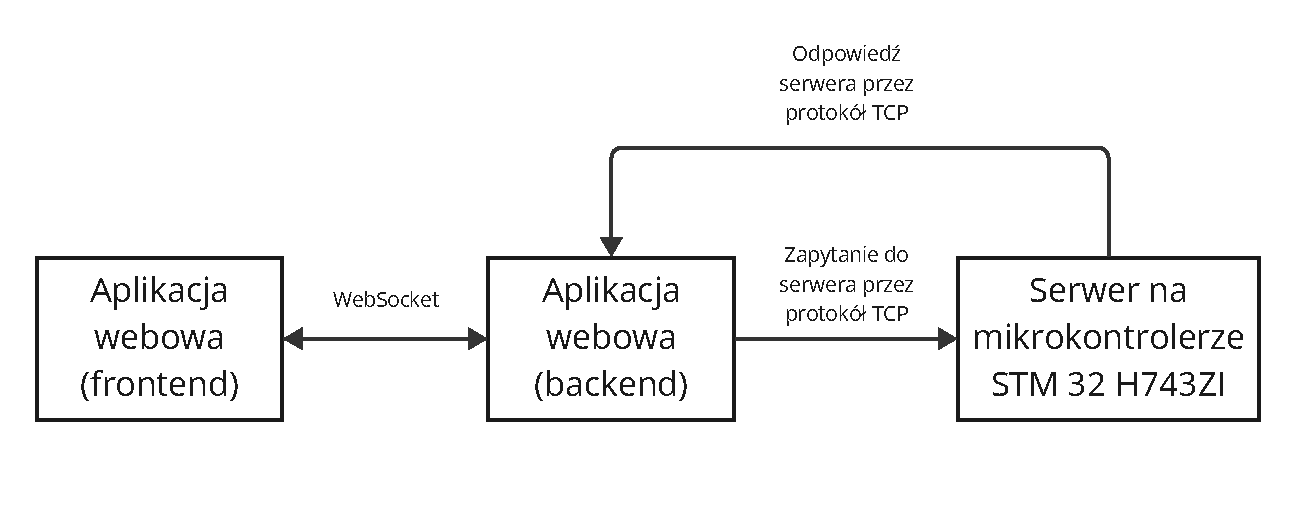
\includegraphics{interface/schemat blokowy.pdf}}
    \caption{Schemat blokowy wymiany danych.}
    \label{fig:schemat blokowy komunikacji ogolny}
\end{figure}
\section{Właściwości TCP}
Protokół TCP posiada wiele zalet:
\begin{enumerate}
    \item \textbf{Niezawodność przesyłu danych:} protokół TCP gwarantuje przesył danych do odbiorcy w oryginalnej formie. Wykorzystuje takie mechanizmy jak numeracja sekwencyjna, potwierdzenie ACK (odbiorca potwierdza otrzymanie pakietu) i retransmisje. W przypadku utraty pakietu, zostanie on przesłany ponownie, aż do otrzymania pełnych danych.
    \item \textbf{Komunikacja dwukierunkowa:} TCP polega na komunikacji dwukierunkowej. Dzięki czemu obydwie strony mogą przesyłać dane. Jest to przydatne w celu potwierdzenia czy odbiorca otrzymał pakiety.
\end{enumerate}
Oprócz swoich korzyści powszechnie stosowany protokół TCP niesie ze sobą niebezpieczeństwa, które mogą go wykluczyć z użytku w aplikacjach.
\begin{enumerate}
    \item \textbf{Podatność na ataki:} jednym z możliwych ataków jest man-in-the-middle, który może prowadzić do przechwycenia i modyfikacji danych bez wiedzy serwera i klienta. Innym przykładem jest atak typu TCP spoofing, polega on na podszyciu się pod innego użytkownika, wysyłając pakiety TCP z fałszywym IP. Może to prowadzić do przechwycenia wrażliwych danych lub złośliwego wstrzyknięcia poleceń.
    \item \textbf{Brak szyfrowania:} protokół TCP nie ma wbudowanego mechanizmu szyfrowania, ani autoryzacji. W związku z tym dane mogą być narażone na podsłuch przez osoby trzecie.
\end{enumerate}
Aplikacja webowa działa tylko lokalnie, dlatego nie trzeba rozpatrywać kwestii bezpieczeństwa. Dobrze zabezpieczona sieć rozwiązuje powyższe problemy.
\section{React}
\label{section:React}
Do zaprogramowania frontendu aplikacji webowej został wybrany React \cite{React}. Jest to biblioteka JavaScript, stworzona i rozwijana przez firmę Meta (dawniej Facebook), która służy do budowania interfejsów użytkownika. Główną zaletą React'a jest obsługa złożonych i dynamicznych aplikacji webowych poprzez użycie komponentów, które mogą być wielokrotnie używane.

\subsection{Działanie Reacta}
React działa według zasady \textbf{Virtual DOM} opisanej w sekcji \ref{section:Virtual DOM}, co oznacza, że zmiany w interfejsie użytkownika są najpierw dokonywane w specjalnej wirtualnej reprezentacji DOM, a dopiero potem synchronizowane z rzeczywistym DOM, co znacznie zwiększa wydajność aplikacji.
\subsection{Zalety Reacta}

\begin{enumerate}
    \item \textbf{Komponenty wielokrotnego użytku}: React pozwala na budowanie aplikacji za pomocą małych izolowanych komponentów, które są zaprojektowane do wielokrotnego użytku i łatwego zarządzania.
    \item \textbf{Wysoka wydajność}: React zawdzięcza swoją wydajność dzięki Virtual DOM. React minimalizuje liczby operacji na rzeczywistym DOM, co przekłada się na wysoką wydajność i szybkość działania aplikacji.
    \item \textbf{Popularność i wsparcie}: React jest popularny na skale światową co wpływa na ogromną społeczność developerów, którzy udostępniają dużą ilość bibliotek, narzędzi oraz wsparcia w przypadku luk w bibliotekach.
    \item \textbf{Możliwość używania JSX}: Jednym z największych plusów React'a jest JSX, rozszerzenie składni JavaScriptu, który umożliwia pisanie kodu podobnego do HTML co znacząco ułatwia tworzenie komponentów i zarządzanie nimi.
    \item \textbf{Ekosystem}: React posiada bogaty ekosystem, w tym React Hooks, który znacznie ułatwia zarządzanie stanem aplikacji.
\end{enumerate}

\subsection{React Hooks}
Hooki to funkcje, które zostały wprowadzone do React od wersji 16.8 i pozwalają na używanie kontroli stanu oraz innych funkcji w komponentach funkcyjnych. Wcześniej całe komponenty trzeba było pisać w klasach, co znacząco utrudniało minimalizm przy małych komponentach. Dzięki hook'om można w prosty sposób zarządzać komponentami.

\begin{enumerate}
    \item \textbf{useState}: pozwala na zarządzanie stanem w komponencie funkcyjnym. Przechowuje aktualne dynamiczne dane, takie jak wprowadzony tekst czy stan przycisku. W aplikacji webowej jest między innymi używany do przechowywania próbek, informacji o pozycji w polach tekstowych czy o stanie przycisku. W przypadku zmiany stanu, komponent w którym został zmieniony stan, jak i komponenty dzieci (ang. \textit{children}), zostaną przeładowane. W przypadku zbyt dużej ilości dzieci, może dojść do problemu z wydajnością. W aplikacji ilość dzieci została ograniczona, dodatkowo zostały zastosowane inne techniki optymalizacyjne, które zostaną opisane w następnych punktach.
    
    \item \textbf{useEffect}: służy do zarządzania efektami ubocznymi w komponencie. Efekty uboczne to operacje, które mają wpływ na zewnętrzne środowisko komponentu. W kontekście wykresów, chodzi o zmianę jednostki i zmianę aktualnych próbek. Jeśli chodzi o główną część aplikacji, to useEffect obsługuje połączenie się z WebSocketem jak i zamknięciem komunikacji.
    
    \item \textbf{useMemo}: służy do optymalizacji wydajności poprzez zapamiętywanie wyników kosztownych obliczeń. Dzięki temu nie musimy co każde odświeżenie stanu ponownie obliczać niektórych danych np. takich jak przekształcenie próbek na inne jednostki np. na radiany. Ten hook działa jak pamięć podręczna dla obliczeń. Ponowne obliczenie tych wartości zachodzi przy zmianie zależności.
    
    \item \textbf{useRef}: pozwala na tworzenie odwołań do elementów DOM oraz przechowywania zmiennych. Różni się od useState tym, że nie wywołuje ponownego przeładowania komponentu. W tym przypadku jest przechowywane połączenie z WebSocketem.
\end{enumerate}
\subsection{React-plotlyjs}
React-plotly.js to biblioteka umożliwiająca integrację biblioteki Plotly.js z Reactem. Służy ona do wizualizacji danych z aplikacjami stworzonymi w React. Umożliwia ona tworzenie zaawansowanych i interaktywnych wykresów, które można w bardzo prosty sposób zarządzać i dynamicznie zmieniać wyświetlane dane na wykresie za pomocą React.
\subsection{Działanie React-plotly}
React-plotly.js oferuje komponent Reactowy, który opiera się na Plotly.js. Wykorzystuje właściwości props, czyli danych o specjalnym kluczu, do definiowania danych, wyglądu i funkcji interaktywnych wykresów. Dzięki tym narzędziom można w prosty sposób sposób zmieniać dane jak i wygląd wykresów. W aplikacji jest możliwość zmiany jednostek, wspomniana wcześniej biblioteka w prosty sposób umożliwia modyfikacji opisów osi jak i zamianę danych na wykresie.
\subsection{Zalety react-plotlyjs}
\begin{enumerate}
    \item \textbf{Interaktywność:} Zapewnia interaktywne funkcje, takie jak powiększanie, przesuwanie, tooltipy i zapis wykresu.
    \item \textbf{Integracja z React:} Dzięki komponentowi plotly.js można w prosty sposób zarządzać dynamicznie stanem wykresów. W tym przypadku cały czas wykresy są aktualizowane z aktualną pozycją rotorów jak i uchybem.
    \item \textbf{Wydajność:} W aplikacji jest wgrywanych, na pojedynczy wykres, co sekundę aż 1 000 nowych próbek, co w znaczny sposób obciąża aplikację. Jednym ze sposobów polepszenia wydajności jest zastosowanie WebGL, poprzez typ wykresu scatterg, co znacząco polepsza wydajność przy renderowaniu wykresów.
    \item \textbf{Eksport danych:} Umożliwia eksport wykresów w formacie PNG.
\end{enumerate}
Standardowe wykresy rozproszone w Plotly.js (\textit{scatter}) wykorzystują SVG do renderowania punktów i linii, co jest efektywne dla małych i średnich zbiorów danych. Na wykresach jest ładowana duża ilość próbek, która może być liczona w milionach przez co w tym przypadku renderowanie za pomocą SVG jest niewydajne. W takich przypadkach wykorzystuje się scattergl, który wykorzystuje WebGL.
Jednym z minusów scattergl jest mniejsza ostrość, ponieważ wykres nie jest renderowany wektorowo.
\section{Komunikacja z aplikacji webowej do STM32}
Do komunikacji jako schemat wiadomości został wybrany \textbf{JSON} (JavaScript Object Notation). JSON jest lekkim formatem danych, który jest zarówno łatwy do odczytania jak i rozszerzenia w razie potrzeby przesłania większej ilości danych. Został szerzej opisany w sekcji \ref{section:JSON}. Przykład komunikacji został przedstawiony na schemacie blokowym \ref{fig:schemat blokowy komunikacji z aplikacji webowej do serwera na STM32}.
\begin{lstlisting}[caption=Przykład struktury JSON z aplikacji webowej do STM32]
{
  "isFetching": 0 || 1,
  "isEngineEnabled": 0 || 1,
  "positionX": int,
  "positionY": int,
  "mode": int {0, 1, 2}
}
\end{lstlisting}
Oznaczenie \textbf{0 || 1} reprezentuje wartości logiczne \textbf{0} (fałsz) lub \textbf{1} (prawda). 
Takie podejście wynika z faktu, że język C domyślnie nie posiada wbudowanego typu \textbf{bool}. 
W przypadku STM32 oraz biblioteki cJSON, opisanej w sekcji \ref{section:cJSON}, dostępne są ich własne implementacje typu logicznego (bool). 
Aby zintegrować obie technologie, znacznie łatwiej jest obsługiwać wartości logiczne jako numeryczne typu \textbf{int}.
\begin{enumerate}
    \item \textbf{isFetching}: informacja dla mikrokontrolera czy ma zapamiętywać odczytaną pozycję w pamięci. W przypadku wartości 1 próbki będą zapisywane w buforze. Analogicznie, dla wartości 0 próbki nie będą zapisywane.
    \item \textbf{isEngineEnabled}: w przypadku wartości 1, obydwa silniki krokowe sterujące osiami się załączą, również aktywuje się możliwość zmiany stanu \textit{CLK}. Analogicznie w przypadku wartości 0 sygnały \textit{CLK} nie będą zmieniać stanu jak i sygnały \textit{ENABLED} będą ustawione na stan niski. Jest to niezwykle przydatne w celu ograniczenia zużycia energii przez silniki jak i przez sterownik w stanie bezczynności.
    \item \textbf{positionX, positionY}: wartość zadana dla osi X i Y, które odpowiadają kątom $q_1$ i $q_2$. Wartość jest przesyłana w formacie \textbf{RAW}, czyli taką jaką enkoder odczytuje. Przesyłanie pozycji w tej formie jest najprostszym rozwiązaniem, ponieważ nie musimy na mikrokontrolerze przetwarzać wartości na inny format. Podczas sterowania silnikiem sprawdzamy aktualną pozycję enkodera, dlatego ustawienie wartości zadanej w tych samych jednostkach, co pomiary dostarczane przez enkoder, ogranicza zamianę wartości na inny format i unika błędów obliczeniowych podczas zamiany formatu. 
    \item \textbf{mode:} tryb sterowania osiami. Dla następujących wartości osie przyjmują następująca trajektorię:
    \begin{itemize}
        \item 0: punkt. Różne wartości punktowe dla dwóch osi.
        \item 1: sinusoidalną.
        \item 2: prostokątną.
    \end{itemize}
\end{enumerate}

\begin{figure}[H]
    \centering
    \resizebox{15.5cm}{!}{
    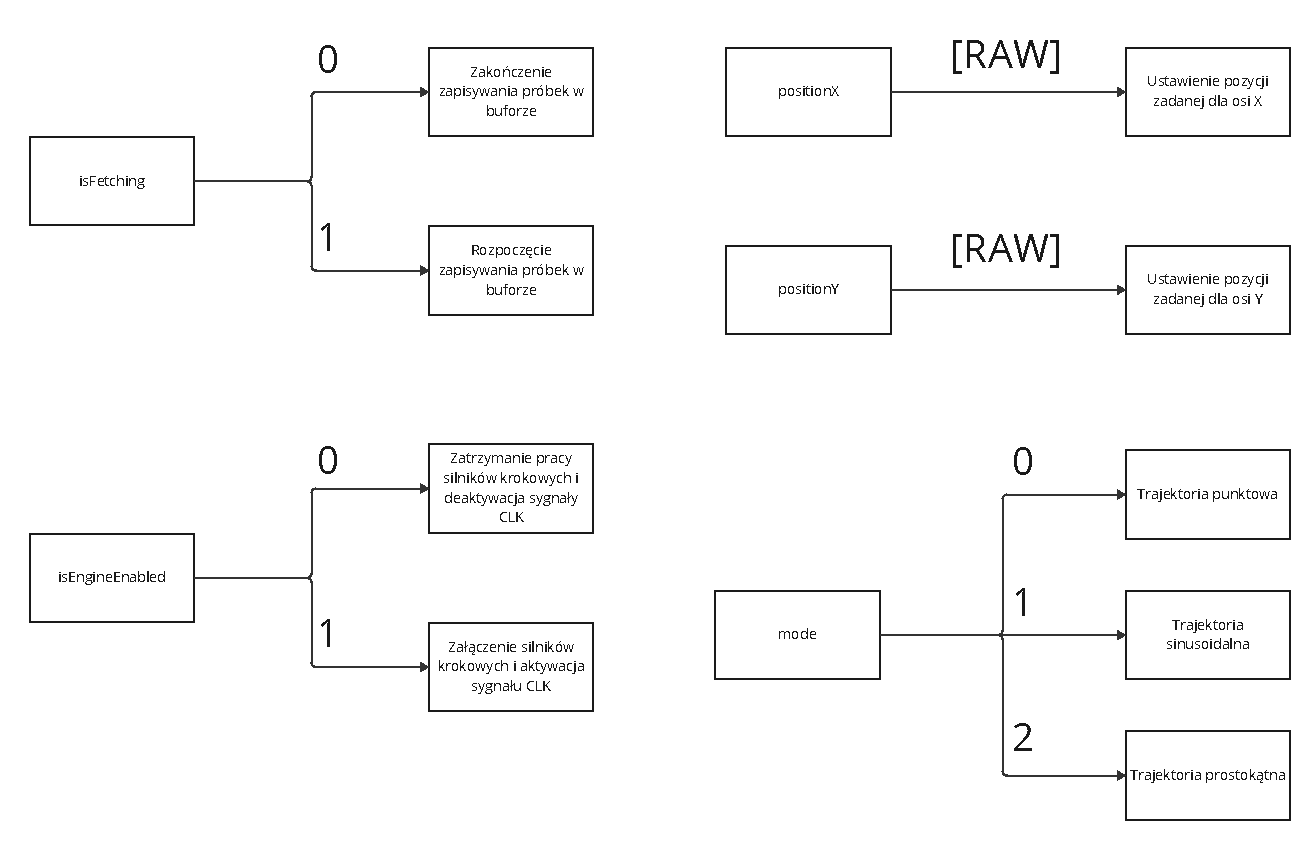
\includegraphics{interface/schemat blokowy json webowa.pdf}}
    \caption{Schemat blokowy struktury JSON z aplikacji webowej.}
    \label{fig:schemat blokowy komunikacji z aplikacji webowej do serwera na STM32}
\end{figure}

W trakcie przesyłania wiadomości nie trzeba przesyłać wszystkich kluczy z wartościami, serwer na STM32 przetworzy tylko wysłane dane. Jest to przydatne w celu zmniejszenia rozmiaru wiadomości oraz ograniczenia błędów w przypadku nie wysłania kluczy ze wszystkimi wartościami. \\
String przesyłany z aplikacji webowej jest na tyle mały, że nie trzeba rozważać przesyłania jednej wiadomości w paru fragmentach (ang. \textit{chunks}).

\section{Komunikacja z STM32 do aplikacji webowej}
Do komunikacji z STM32 do aplikacji webowej również został wybrany format danych typu \textbf{JSON}. Przykład komunikacji został przedstawiony na schemacie
blokowym \ref{fig:schemat blokowy odpowiedzi serwera na STM32}.
\begin{lstlisting}[caption=Przykład struktury JSON z STM32 do aplikacji webowej, label={lst:json_exampleSTM32}]
{
  "dataX": [int],
  "dataY": [int],
  "dataErrorX": [int],
  "dataErrorY": [int]
}
\end{lstlisting}
\begin{enumerate}
    \item \textbf{dataX:} Odczytane próbki z osi X w formacie RAW.
    \item \textbf{dataY:} Odczytane próbki z osi Y w formacie RAW.
    \item \textbf{dataErrorX:} Uchyb na osi X w formacie RAW.
    \item \textbf{dataErrorY:} Uchyb na osi Y w formacie RAW.
\end{enumerate}

\begin{figure}[H]
    \centering
    \resizebox{6cm}{!}{
    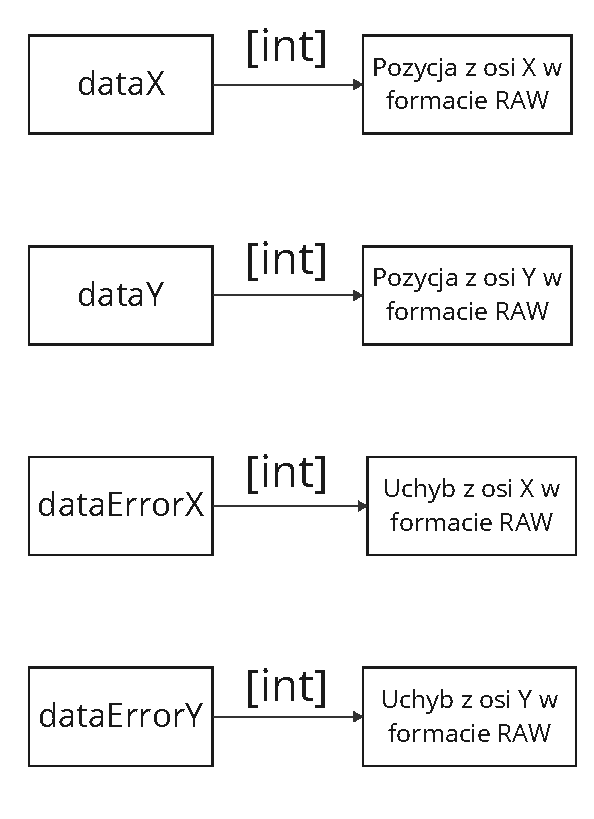
\includegraphics{interface/schemat blokowy json stm32.pdf}}
    \caption{Schemat blokowy odpowiedzi struktury JSON z serwera na STM32.}
  \label{fig:schemat blokowy odpowiedzi serwera na STM32}
\end{figure}
Aby przekształcić wartość z enkodera wyrażoną w jednostkach RAW na stopnie kątowe, należy pomnożyć ją przez 3.428374026619764e-7.  
W celu uzyskania radianów wartość RAW należy pomnożyć przez 5.98364147543706e-9.\\
Przesyłany ciąg znaków może być na tyle duży, że wiadomość zostanie podzielona na dwie lub więcej części. W związku z tym konieczne jest buforowanie fragmentów, ich łączenie oraz sprawdzanie, czy cała wiadomość została już odebrana. Ciąg znaków zawsze kończy się znakiem "\textbf{\}}", co ułatwia identyfikację końca wiadomości i umożliwia poprawne łączenie fragmentów.